\documentclass[12pt, fullpage]{article}
\usepackage{amssymb,latexsym,amsmath,amscd,epsfig,amsthm,graphicx}
\newcommand*{\QEDA}{\hfill\ensuremath{\blacksquare}}%
\pagestyle{empty}

\input epsf
\newdimen\epsfxsize

\parindent=0pt
\setlength{\evensidemargin}{0.0cm}
\setlength{\oddsidemargin}{-1.7cm}
\setlength{\topmargin}{-3.2cm}
%\setlength{\baselineskip}{20pt}
\setlength{\textwidth}{19cm}
\setlength{\textheight}{23cm}

\newcommand{\ds}{\displaystyle}
\newcommand{\un}{\underline}
\newcommand{\R}{\mathbb R}


\begin{document}
\begin{flushleft}
\textbf{Nilay Bhatt Feb. 8 2017}		
\end{flushleft}
\begin{center}
	\textbf{Results about Euler's path and circuits}
\end{center}
\begin{center}
		
{\bf MATH 450 Seminar in Proof}
 \\
\end{center}
\textbf{Definition 1.1: \textit{Euler Path: }}An \textit{Euler Path} on a graph $G$ is a path that traverses each edge exactly once.\\
\textbf{Definition 1.2: \textit{Euler Circuit/Cycle: }}An Euler circuit on a graph $G$ is a Euler Path which starts and ends on the same node.\\ \\
\textbf{Results to be proven: }

\begin{enumerate}
	\item Show that any graph where the degree of every vertex is even iff it has an Eulerian circuit.
	\item Show that if there are exactly two vertices a and b of odd degree, there is an Eulerian path on the graph.
\end{enumerate}
$Proof:$
\begin{enumerate}
	\item
 	$\Rightarrow$ Let $G$ be a graph such that it has an Euler circuit. According to the definition of Euler Circuit on a graph, given a vertex $v_1$, we can traverse every other node only once and end at the vertex $v_1$. Thus every node/vertex has one entry point and one exit point. We know this because $G$ has an Euler circuit. Thus every node/vertex has two edges attached to it thus making it a node of even degree. \\
 	$\Leftarrow$ Let every node in a graph $G$ have an even degree. Let us prove this by induction. Assume, that there are only two nodes in $G$, each with two edges on them. Thus it is clear that you will end on the same node that you started with, thus making a Euler circuit on $G$. \\
 	Now,let $G$ be  graph of even degree with more than two nodes. Lets start with an arbitrary node $v_1$. Now since every node has an even degree, we can follow a trail from $v_1$ to the next node and repeat it for the next node we encounter. We know that this is possible because each time we enter a node $v_k$ we know there is an unused edge adjacent to it for us to use to traverse. Thus using a unique path we will come back on $v_1$ since there are even number of edges, we will always find an untapped edge to let us continue our path back to $v_1$.
\begin{figure}[h!]
  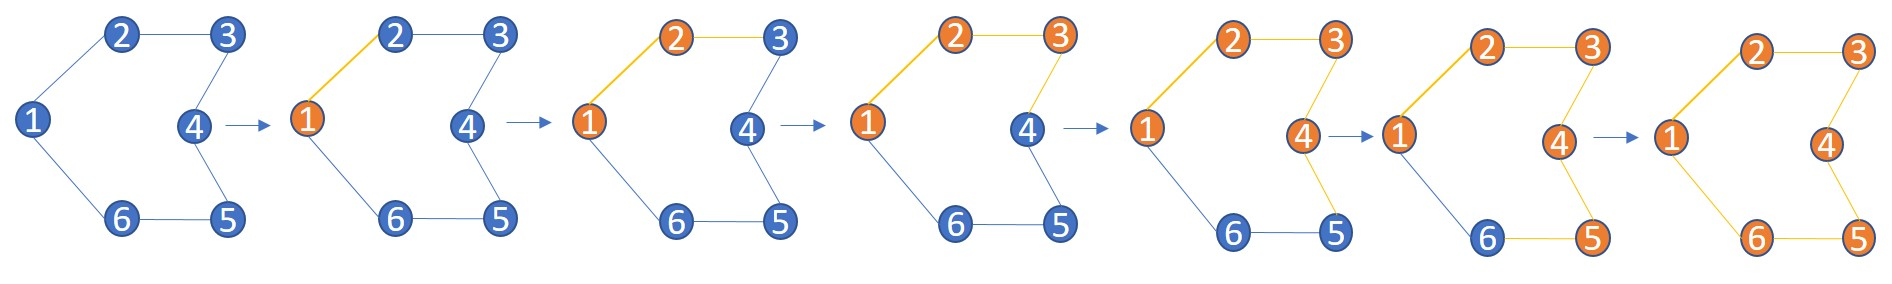
\includegraphics[width=\linewidth	]{circuit.jpg}
  \caption{A Euler Circuit.}
  \label{fig:ec1}
\end{figure} 	
 	Figure 1. \ref{fig:ec1}Euler Circuit
	\item
	Let $G$ be a graph with Euler circuit. Thus every node/vertex has an even degree. now let us add one node say $b$ and add an edge to a node $a$ in the existing graph $G$. Note that before adding the edge from $b$ to $a$, $a$ in $G$ had an even degree. Now if we start drawing our path from $b$, and since it has only one edge connecting to $a$ we go to $a$ now, if we hypothetically ignore the edge connecting $a$ and $b$, the remainder of $G$ has nodes with even edges, thus making it a Euler circuit. Therefore, the trail will end at $a$ but since we have already used the edge connecting $a$ and $b$, we stop at $a$. Thus we were able to traverse all the edges in $G$ +$b$ exactly once, starting from $b$ and ending at an edge $a$ in $G$.
\end{enumerate}

\QEDA

\end{document}